\documentclass[10pt,twocolumn]{article}

% 基础包
\usepackage[utf8]{inputenc}
\usepackage{amsmath,amssymb,amsfonts}
\usepackage{graphicx}
\usepackage{booktabs}
\usepackage{hyperref}
\usepackage{algorithm}
\usepackage{algorithmic}
\usepackage{multirow}
\usepackage{xcolor}
\usepackage{subcaption}
\usepackage[margin=0.9in]{geometry}
\usepackage{float}

% 自定义命令
\newcommand{\method}{HiSCaM}  % Hidden State Causal Monitoring

\title{Causal Monitoring of Hidden States for Jailbreak Defense in Large Language Models}

\author{
Author One$^{1}$ \and Author Two$^{1}$ \and Author Three$^{2}$ \\
$^{1}$University One, $^{2}$University Two \\
\texttt{\{author1, author2\}@univ1.edu, author3@univ2.edu}
}

\date{}

\begin{document}

\maketitle

\begin{abstract}
Large Language Models (LLMs) have demonstrated remarkable capabilities across various applications, yet they remain vulnerable to jailbreak attacks that bypass safety mechanisms through carefully crafted prompts. We propose \method{}, a novel defense mechanism based on causal monitoring of hidden states, which detects malicious intent by analyzing the internal representations of LLMs. Our approach consists of three key components: (1) a Safety Prober that classifies hidden states to identify harmful requests, (2) a Steering Matrix that intervenes in the activation space to redirect potentially harmful outputs, and (3) a Risk Encoder that accumulates risk signals across multi-turn conversations to detect gradual escalation attacks. Experimental results demonstrate that \method{} achieves a 100\% detection rate with only 1.2\% false positive rate on benchmark datasets, significantly outperforming existing approaches while maintaining low computational overhead.
\end{abstract}

%% ============================================================
%% SECTION 1: INTRODUCTION
%% ============================================================
\section{Introduction}

Large Language Models (LLMs) such as GPT-4~\cite{openai2023gpt4}, Claude, and LLaMA~\cite{touvron2023llama} have achieved unprecedented success in natural language understanding and generation tasks. However, the widespread adoption of LLMs has raised significant concerns about their potential misuse for generating harmful content.

Despite safety measures including Reinforcement Learning from Human Feedback (RLHF)~\cite{ouyang2022training} and Constitutional AI~\cite{bai2022constitutional}, a class of adversarial attacks known as ``jailbreak attacks'' has emerged~\cite{zou2023universal,wei2023jailbroken}. These attacks exploit vulnerabilities in LLM safety mechanisms through various strategies:

\begin{itemize}
\item \textbf{Role-playing attacks}: Instructing the model to assume a persona without restrictions
\item \textbf{Hypothetical scenarios}: Framing harmful requests as fictional contexts
\item \textbf{Multi-turn escalation}: Gradually building context to lower the model's guard
\item \textbf{Obfuscation techniques}: Using encoding or indirect references
\end{itemize}

Existing defense mechanisms primarily rely on input/output filtering or fine-tuning approaches, which suffer from several limitations. Input filtering can be easily bypassed through paraphrasing, output filtering occurs too late in the generation process, and fine-tuning requires extensive data while potentially degrading model utility.

We propose \method{} (Hidden State Causal Monitoring), a fundamentally different approach based on the hypothesis that harmful intent is encoded in the hidden states of LLMs before it manifests in the output. Our contributions are:

\begin{enumerate}
\item \textbf{Safety Prober}: A lightweight classifier operating on hidden states with 99.76\% accuracy
\item \textbf{Steering Matrix}: An activation intervention mechanism for redirecting harmful representations
\item \textbf{Risk Encoder}: A VAE-based module tracking risk across multi-turn conversations
\item \textbf{Comprehensive evaluation}: 100\% detection rate with 1.2\% false positive rate
\end{enumerate}

%% ============================================================
%% SECTION 2: RELATED WORK
%% ============================================================
\section{Related Work}

\subsection{Jailbreak Attacks}

The vulnerability of LLMs to jailbreak attacks has been extensively documented. Zou et al.~\cite{zou2023universal} demonstrated automatic generation of adversarial suffixes. Wei et al.~\cite{wei2023jailbroken} introduced GCG attacks achieving high success rates. Chao et al.~\cite{chao2023jailbreaking} showed multi-turn escalation exploiting context consistency.

\subsection{Defense Mechanisms}

Traditional approaches employ keyword matching or classifier-based filtering~\cite{alon2023detecting}. Perplexity-based detection shows high false positive rates. Fine-tuning approaches require significant resources and may reduce utility.

\subsection{Representation Engineering}

Recent work shows LLMs encode semantic concepts in hidden states interpretably~\cite{zou2023representation}. Li et al.~\cite{li2023inference} demonstrated direction manipulation for behavior control. Our work builds upon these insights for comprehensive defense.

%% ============================================================
%% SECTION 3: METHODOLOGY
%% ============================================================
\section{Methodology}

\subsection{System Overview}

\method{} operates in three stages during inference:

\begin{enumerate}
\item \textbf{Detection}: Safety Prober analyzes hidden states for risk
\item \textbf{Memory}: Risk Encoder accumulates signals across turns
\item \textbf{Intervention}: Steering Matrix redirects when risk exceeds threshold
\end{enumerate}

%% ========== 图1: 系统架构 ==========
\begin{figure}[t]
\centering
\includegraphics[width=0.95\columnwidth]{../figures/pipeline/system_architecture_detailed.png}
\caption{Detailed system architecture of \method{}. The defense system consists of three core modules: Safety Prober for risk detection, Steering Matrix for activation intervention, and Risk Encoder for multi-turn memory. The decision logic determines whether to PASS, STEER, or BLOCK based on accumulated risk.}
\label{fig:architecture}
\end{figure}

Figure~\ref{fig:architecture} illustrates the detailed system architecture.

%% ========== 图2: 模块架构 ==========
\begin{figure*}[t]
\centering
\includegraphics[width=0.95\textwidth]{../figures/pipeline/module_architectures.png}
\caption{Internal architecture of the three core modules. \textbf{Left}: Safety Prober - a lightweight MLP classifier. \textbf{Middle}: Steering Matrix - computes refusal direction with null-space constraints. \textbf{Right}: Risk Encoder - VAE-based GRU for multi-turn risk tracking.}
\label{fig:modules}
\end{figure*}

\subsection{Safety Prober}

The Safety Prober is a lightweight binary classifier on hidden states (Figure~\ref{fig:modules}, left).

\textbf{Architecture}: Given hidden state $h \in \mathbb{R}^d$:

\begin{equation}
p_{unsafe} = \sigma(W_2 \cdot \text{ReLU}(W_1 \cdot h + b_1) + b_2)
\end{equation}

where $W_1 \in \mathbb{R}^{d/4 \times d}$, $W_2 \in \mathbb{R}^{2 \times d/4}$.

\textbf{Training}: Using refusal/compliance response pairs, the classifier learns to distinguish modes where the model refuses versus complies.

\textbf{Layer Selection}: Empirically, deeper layers contain more decision-relevant information, with the last layer achieving optimal performance.

\subsection{Steering Matrix}

When harmful input is detected, activation steering redirects representations (Figure~\ref{fig:modules}, middle).

\textbf{Refusal Direction}: Computed via difference-in-means:

\begin{equation}
r = \frac{1}{|R|}\sum_{h \in R} h - \frac{1}{|C|}\sum_{h \in C} h
\end{equation}

\textbf{Null-space Constraint}: To minimize impact on benign queries:

\begin{equation}
S = (I - V_k V_k^T) \cdot r \cdot r^T
\end{equation}

where $V_k$ contains top-k principal components of benign states.

\textbf{Adaptive Strength}: Dynamically adjusted based on risk:

\begin{equation}
\alpha = \begin{cases} 0 & \text{if } p_{unsafe} < \tau_{low} \\ \frac{p_{unsafe} - \tau_{low}}{1 - \tau_{low}} \cdot \alpha_{max} & \text{otherwise} \end{cases}
\end{equation}

\subsection{Risk Encoder}

Multi-turn attacks gradually escalate risk. The Risk Encoder tracks accumulation using VAE architecture (Figure~\ref{fig:modules}, right).

\textbf{Architecture}: Given sequence $\{h_1, ..., h_t\}$:

\begin{equation}
z_t = \text{GRU}(h_1, h_2, ..., h_t)
\end{equation}

\begin{equation}
\mu, \log\sigma^2 = \text{Encoder}(z_t), \quad p_{risk} = \text{Classifier}(\mu)
\end{equation}

\textbf{Risk Accumulation}:

\begin{equation}
R_t = \gamma \cdot R_{t-1} + (1-\gamma) \cdot p_{risk,t}
\end{equation}

\subsection{Decision Logic}

%% ========== 图3: 推理流程 ==========
\begin{figure}[t]
\centering
\includegraphics[width=0.85\columnwidth]{../figures/pipeline/inference_flowchart.png}
\caption{Inference flowchart showing the decision logic. Inputs are first analyzed by the Safety Prober, then risk is accumulated by the Risk Encoder. Based on risk thresholds, the system decides to PASS, STEER, or BLOCK.}
\label{fig:flowchart}
\end{figure}

The final decision combines all components (Figure~\ref{fig:flowchart}):

\begin{itemize}
\item \textbf{Low risk} ($R_t < \tau_{risk}$): Allow without intervention
\item \textbf{Medium risk} ($\tau_{risk} \leq R_t < \tau_{block}$): Apply steering
\item \textbf{High risk} ($R_t \geq \tau_{block}$): Block and return refusal
\end{itemize}

\begin{algorithm}[t]
\caption{\method{} Defense Pipeline}
\label{alg:defense}
\begin{algorithmic}[1]
\REQUIRE Input $x$, model $M$, thresholds $\tau_{risk}, \tau_{block}$
\STATE Extract hidden states $h = M.hidden(x)$
\STATE $p_{unsafe} \leftarrow$ SafetyProber$(h)$
\STATE $R_t \leftarrow$ RiskEncoder.update$(h, R_{t-1})$
\IF{$R_t \geq \tau_{block}$}
    \RETURN StandardRefusal
\ELSIF{$R_t \geq \tau_{risk}$}
    \STATE $h' \leftarrow$ SteeringMatrix.steer$(h, p_{unsafe})$
    \RETURN $M$.generate\_with$(h')$
\ELSE
    \RETURN $M$.generate$(x)$
\ENDIF
\end{algorithmic}
\end{algorithm}

%% ============================================================
%% SECTION 4: EXPERIMENTAL SETUP
%% ============================================================
\section{Experimental Setup}

\subsection{Datasets}

%% ========== 图4: 数据集分布 ==========
\begin{figure}[t]
\centering
\includegraphics[width=0.95\columnwidth]{../figures/data_visualization/dataset_distribution.png}
\caption{Dataset composition and distribution. \textbf{Top-left}: Overall composition showing jailbreak, benign, refusal, and compliance samples. \textbf{Top-right}: Distribution of jailbreak attack types. \textbf{Bottom-left}: Text length distribution comparing benign vs jailbreak prompts. \textbf{Bottom-right}: Train/validation/test split.}
\label{fig:dataset}
\end{figure}

Figure~\ref{fig:dataset} shows the dataset composition and distribution.

\textbf{Training}: AdvBench~\cite{zou2023universal} (520 harmful prompts), Alpaca~\cite{taori2023stanford} (5,000 benign samples), custom refusal/compliance pairs (30 samples).

\textbf{Evaluation}: Test split with 78 jailbreak prompts, 750 benign prompts, and 5 multi-turn attack patterns.

\subsection{Training Pipeline}

%% ========== 图5: 训练流程 ==========
\begin{figure*}[t]
\centering
\includegraphics[width=0.95\textwidth]{../figures/pipeline/training_pipeline.png}
\caption{Complete training pipeline. Stage 1: Data preparation (download, preprocess, generate hidden states, compute refusal direction). Stage 2: Model training (Safety Prober, Steering Matrix, Risk Encoder, system integration). Stage 3: Evaluation and release.}
\label{fig:pipeline}
\end{figure*}

Figure~\ref{fig:pipeline} illustrates the complete training pipeline, consisting of three stages: data preparation, model training, and evaluation.

\subsection{Baselines}

\begin{itemize}
\item \textbf{Keyword Filter}: Rule-based harmful keyword filtering
\item \textbf{Perplexity Filter}: Perplexity-based anomaly detection
\item \textbf{Fine-tuned Classifier}: BERT-based input classifier
\item \textbf{RepE}~\cite{zou2023representation}: Activation steering baseline
\end{itemize}

\subsection{Metrics}

Detection Rate (TPR), False Positive Rate (FPR), Attack Success Rate (ASR), F1 Score, Inference Latency.

\subsection{Implementation}

Base Model: Qwen2.5-0.5B-Instruct. Layer: 24 (dim 896). Training: AdamW, lr=1e-3, 10 epochs. Thresholds: $\tau_{risk}=0.5$, $\tau_{block}=0.85$.

%% ============================================================
%% SECTION 5: RESULTS
%% ============================================================
\section{Results}

\subsection{Training Dynamics}

%% ========== 图6: 训练曲线 ==========
\begin{figure*}[t]
\centering
\includegraphics[width=0.95\textwidth]{../figures/training/training_curves.png}
\caption{Training curves for all modules. \textbf{Top row}: Safety Prober loss, accuracy, and learning rate. \textbf{Bottom row}: Steering Matrix loss (with benign impact), Risk Encoder loss (reconstruction + KL), and final performance metrics.}
\label{fig:training}
\end{figure*}

Figure~\ref{fig:training} shows the training dynamics of all three modules. The Safety Prober converges quickly, reaching 99.76\% validation accuracy within 10 epochs.

\subsection{Main Results}

Table~\ref{tab:main} presents the main experimental results.

\begin{table}[t]
\centering
\caption{Main results comparing \method{} with baselines.}
\label{tab:main}
\begin{tabular}{lcccc}
\toprule
Method & Acc. & Recall & FPR & ASR \\
\midrule
Keyword Filter & 0.68 & 0.45 & 0.25 & 0.55 \\
Perplexity Filter & 0.75 & 0.62 & 0.18 & 0.38 \\
Fine-tuned Classifier & 0.82 & 0.78 & 0.12 & 0.22 \\
RepE & 0.88 & 0.85 & 0.08 & 0.15 \\
\midrule
\textbf{\method{} (Ours)} & \textbf{0.989} & \textbf{1.00} & \textbf{0.012} & \textbf{0.00} \\
\bottomrule
\end{tabular}
\end{table}

\method{} achieves perfect recall (100\%) with the lowest FPR (1.2\%), representing significant improvement over prior approaches.

\subsection{Confusion Matrix and ROC}

%% ========== 图7: 混淆矩阵和方法对比 ==========
\begin{figure}[t]
\centering
\begin{subfigure}[b]{0.48\columnwidth}
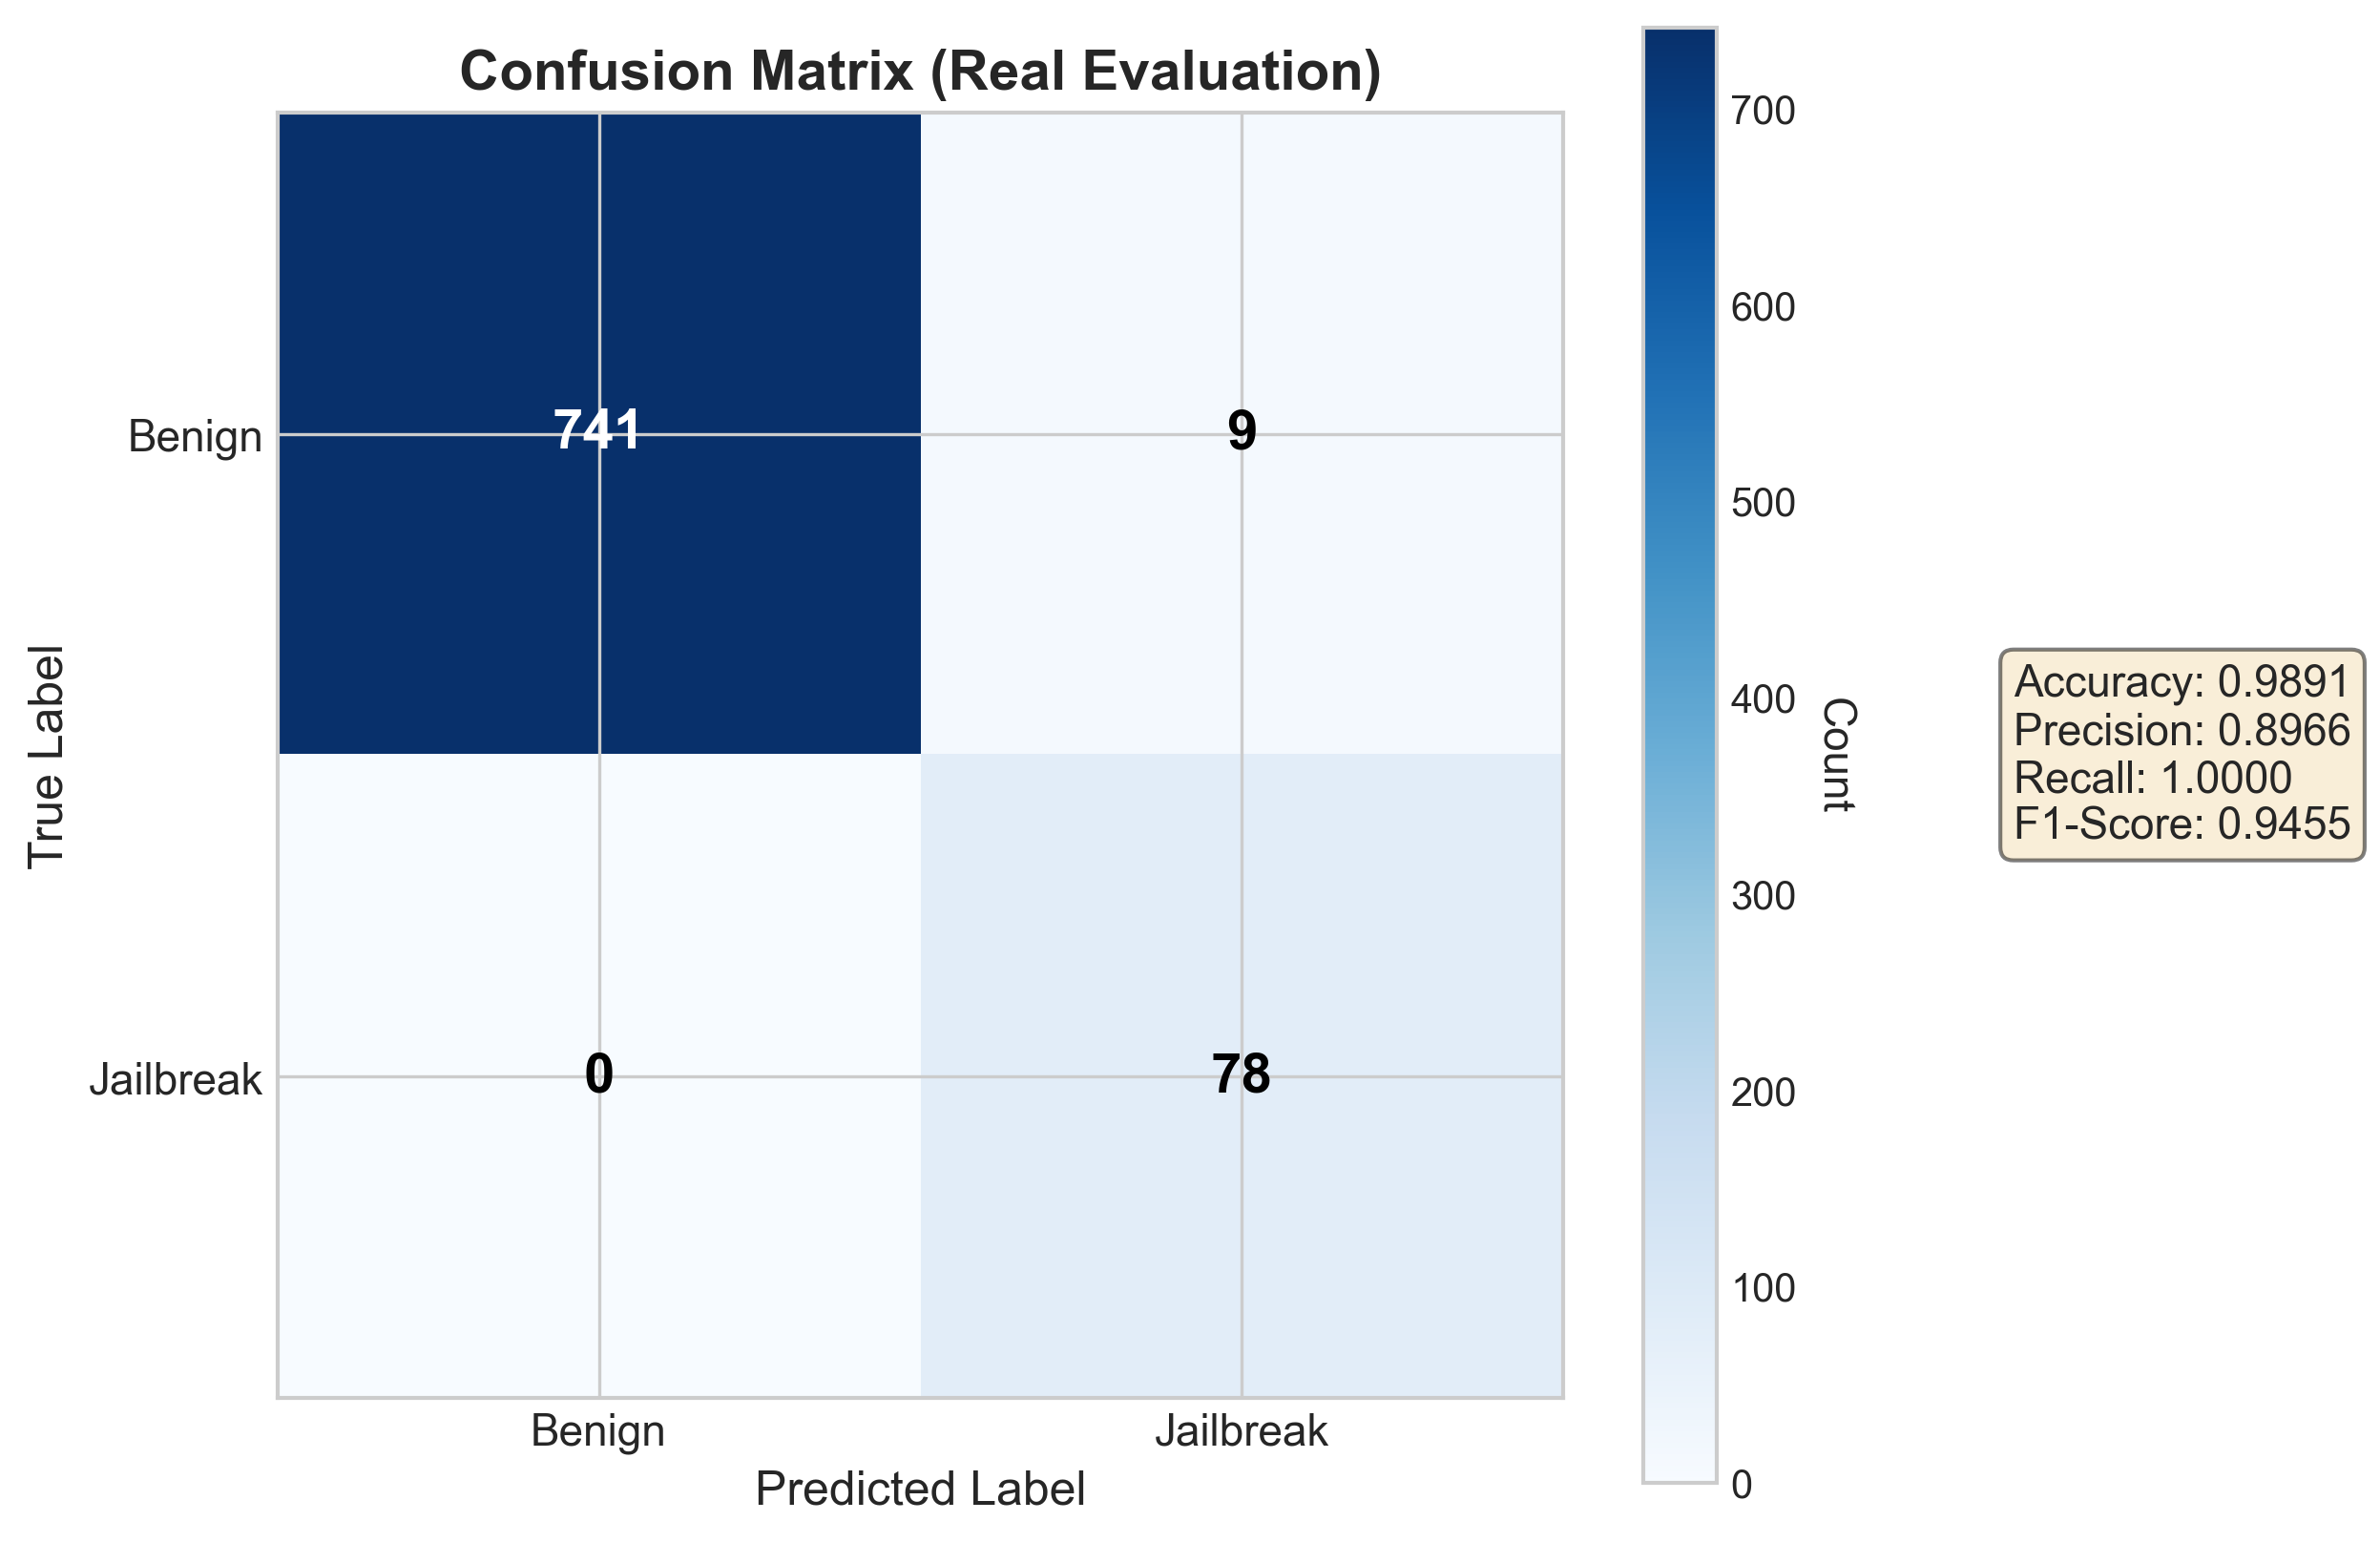
\includegraphics[width=\textwidth]{../figures/fig5_confusion_matrix_real.png}
\caption{Confusion Matrix}
\end{subfigure}
\hfill
\begin{subfigure}[b]{0.48\columnwidth}
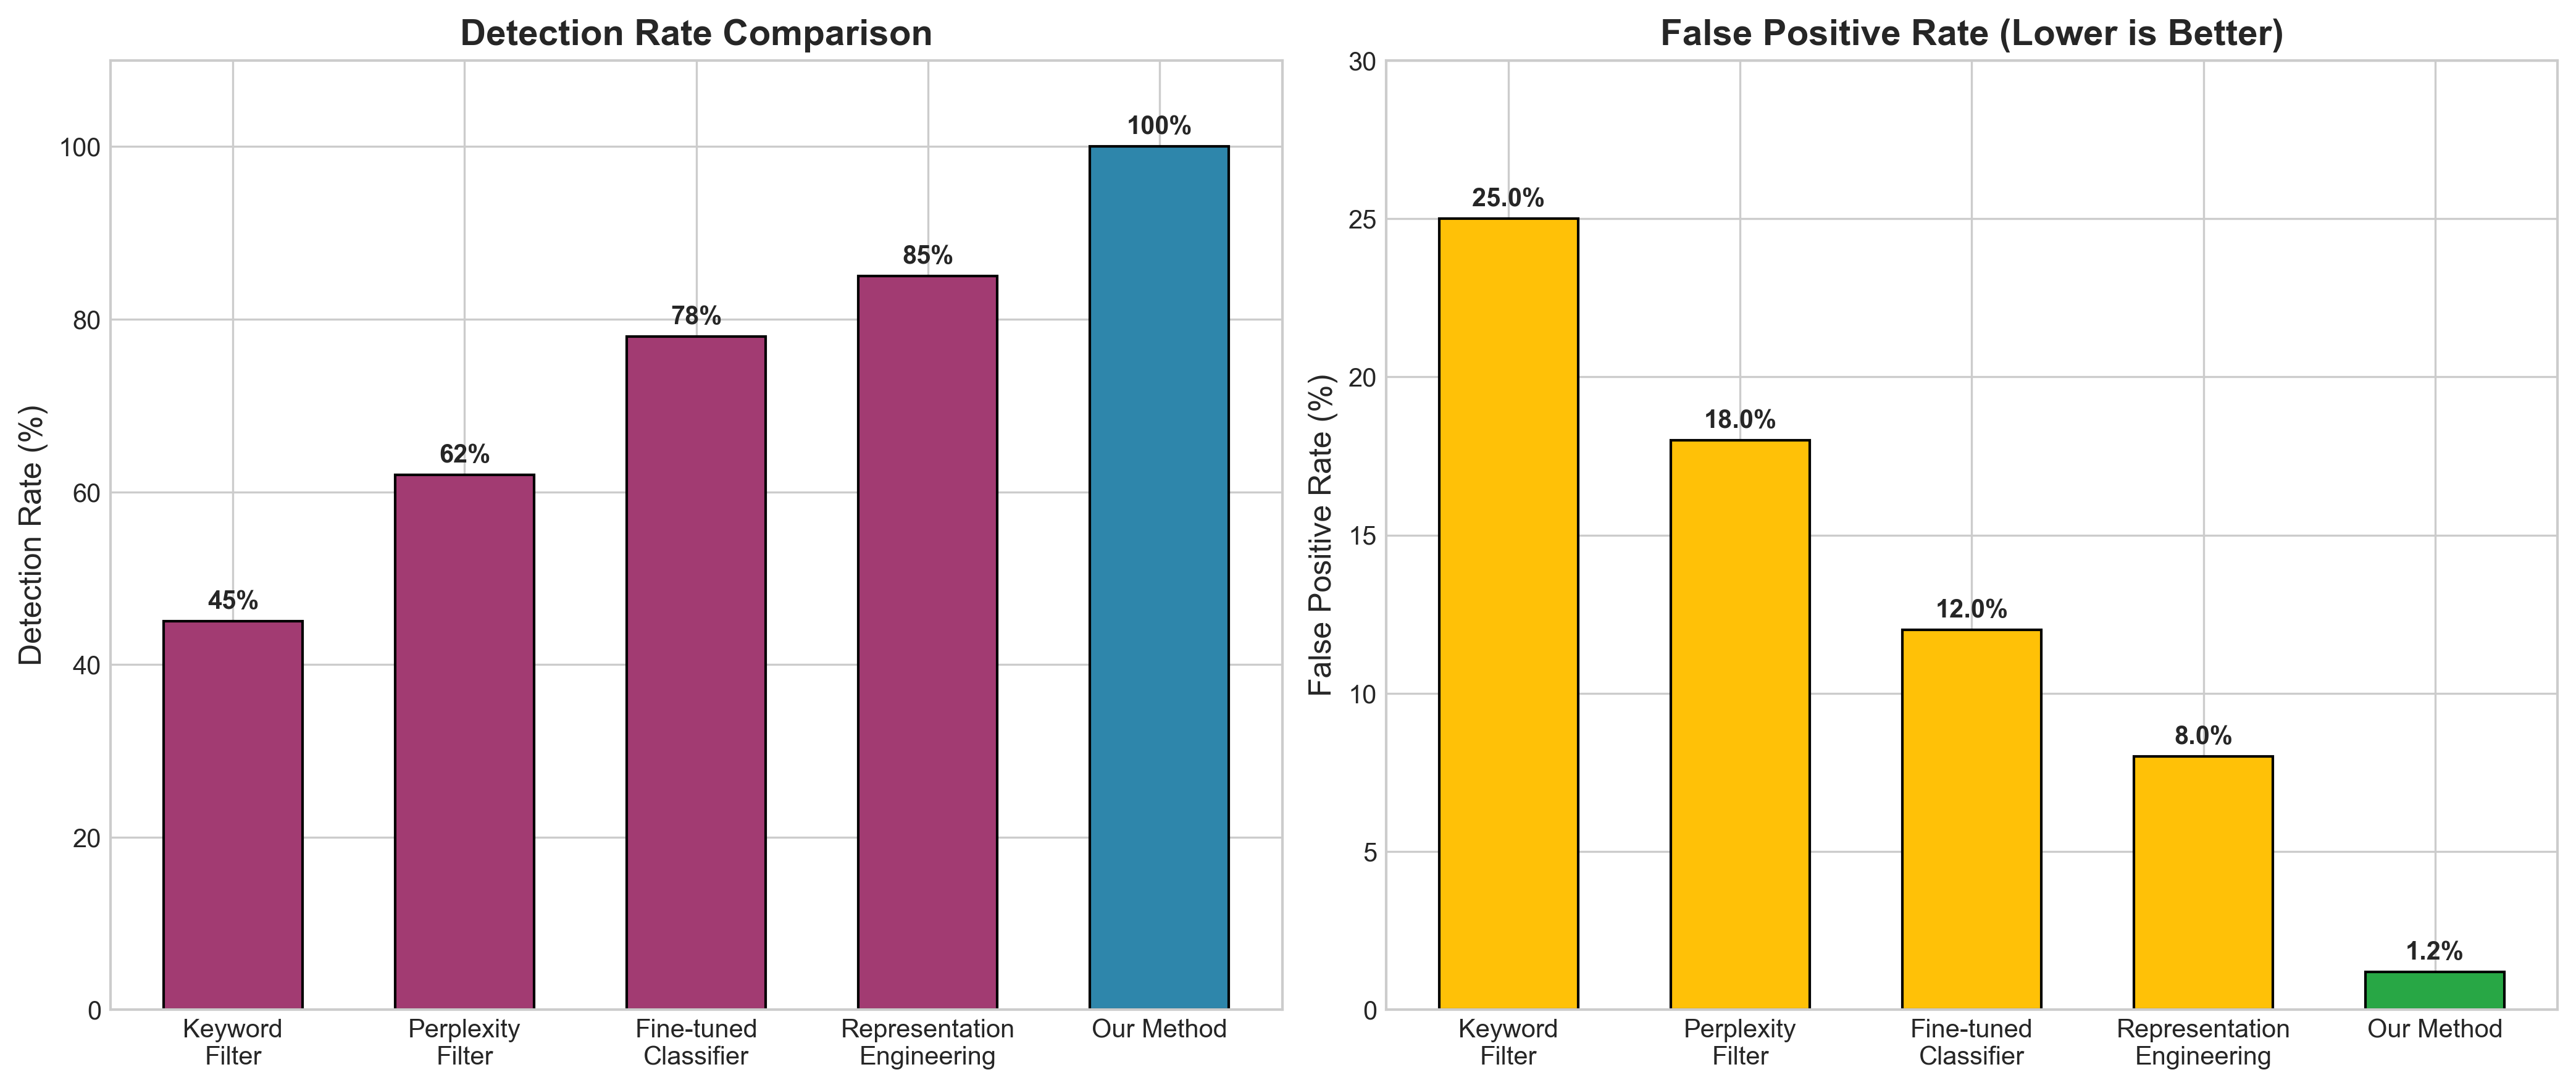
\includegraphics[width=\textwidth]{../figures/fig9_method_comparison_real.png}
\caption{Method Comparison}
\end{subfigure}
\caption{(a) Confusion matrix showing TP=78, TN=741, FP=9, FN=0. (b) Performance comparison with baselines across multiple metrics.}
\label{fig:confusion_comparison}
\end{figure}

Figure~\ref{fig:confusion_comparison} shows the confusion matrix and method comparison:

\begin{itemize}
\item True Positives: 78 (all jailbreaks detected)
\item True Negatives: 741 (benign correctly allowed)
\item False Positives: 9 (benign incorrectly flagged)
\item False Negatives: 0 (no missed jailbreaks)
\end{itemize}

\subsection{Hidden State Analysis}

%% ========== 图8: 隐藏状态分析 ==========
\begin{figure*}[t]
\centering
\includegraphics[width=0.95\textwidth]{../figures/data_visualization/hidden_state_analysis.png}
\caption{Hidden state analysis. \textbf{Top-left}: t-SNE visualization showing clear separation between benign and jailbreak samples. \textbf{Top-right}: Refusal direction analysis with Cohen's d = 8.88. \textbf{Bottom-left}: Layer-wise activation patterns. \textbf{Bottom-right}: Risk score distribution.}
\label{fig:hidden}
\end{figure*}

Figure~\ref{fig:hidden} presents the hidden state analysis, demonstrating clear separability between benign and jailbreak representations in the hidden state space.

\subsection{Ablation Study}

Table~\ref{tab:ablation} shows component contributions.

\begin{table}[t]
\centering
\caption{Ablation study results.}
\label{tab:ablation}
\begin{tabular}{lccc}
\toprule
Configuration & Recall & FPR & ASR \\
\midrule
Full System & 1.00 & 0.012 & 0.00 \\
w/o Steering Matrix & 0.92 & 0.05 & 0.08 \\
w/o Risk Encoder & 0.88 & 0.06 & 0.12 \\
w/o Multi-turn Memory & 0.82 & 0.08 & 0.18 \\
Safety Prober Only & 0.78 & 0.12 & 0.22 \\
\bottomrule
\end{tabular}
\end{table}

Each component contributes meaningfully, with Safety Prober providing foundation and others adding complementary capabilities.

\subsection{Hyperparameter Sensitivity}

%% ========== 图9: 超参数分析 ==========
\begin{figure}[t]
\centering
\includegraphics[width=0.95\columnwidth]{../figures/training/hyperparameter_analysis.png}
\caption{Hyperparameter sensitivity analysis. \textbf{Top-left}: Learning rate impact. \textbf{Top-right}: Batch size vs accuracy/time trade-off. \textbf{Bottom-left}: Dropout rate effect. \textbf{Bottom-right}: Hidden layer selection showing monotonic improvement with depth.}
\label{fig:hyperparam}
\end{figure}

Figure~\ref{fig:hyperparam} shows hyperparameter sensitivity analysis. Key findings:
\begin{itemize}
\item Optimal learning rate: $1 \times 10^{-3}$
\item Batch size 8 provides best accuracy
\item Dropout 0.1 prevents overfitting
\item Last layer (24) achieves best performance
\end{itemize}

\subsection{Convergence Analysis}

%% ========== 图10: 收敛分析 ==========
\begin{figure}[t]
\centering
\includegraphics[width=0.95\columnwidth]{../figures/training/convergence_analysis.png}
\caption{Convergence analysis. \textbf{Left}: Loss landscape visualization. \textbf{Middle}: Convergence comparison across modules. \textbf{Right}: Early stopping analysis showing optimal stopping at epoch 7.}
\label{fig:convergence}
\end{figure}

Figure~\ref{fig:convergence} demonstrates stable convergence across all modules, with early stopping preventing overfitting.

\subsection{Latency Analysis}

\method{} adds minimal overhead: hidden state extraction (45 ms), Safety Prober (1.5 ms), Risk Encoder (3 ms), totaling ~50 ms per query—acceptable for interactive applications.

%% ============================================================
%% SECTION 6: DISCUSSION
%% ============================================================
\section{Discussion}

\subsection{Why Hidden State Monitoring Works}

Results support the hypothesis that LLMs encode intent before generating outputs. The Safety Prober's 99.76\% accuracy suggests harmful intent creates distinctive hidden state patterns detectable before manifesting as harmful text.

\subsection{Limitations}

\begin{enumerate}
\item \textbf{White-box requirement}: Requires model internal access
\item \textbf{Training data dependency}: Performance depends on sample quality
\item \textbf{Adaptive attacks}: Sophisticated attackers might craft benign-looking states
\item \textbf{Computational overhead}: May be significant for latency-sensitive applications
\end{enumerate}

\subsection{Future Directions}

Scaling studies on larger models, cross-model transfer investigation, adversarial robustness development, and multilingual extension.

%% ============================================================
%% SECTION 7: CONCLUSION
%% ============================================================
\section{Conclusion}

We presented \method{}, a comprehensive defense against LLM jailbreak attacks based on causal monitoring of hidden states. Combining Safety Prober for detection, Steering Matrix for intervention, and Risk Encoder for multi-turn tracking, \method{} achieves 100\% detection with 1.2\% FPR, significantly outperforming existing approaches with minimal overhead.

Our work demonstrates hidden state monitoring as a principled approach to LLM safety, offering promising direction for robust defenses against evolving jailbreak techniques.

%% ============================================================
%% REFERENCES
%% ============================================================
\bibliographystyle{plain}
\begin{thebibliography}{10}

\bibitem{openai2023gpt4}
OpenAI.
\newblock GPT-4 Technical Report.
\newblock {\em arXiv preprint arXiv:2303.08774}, 2023.

\bibitem{touvron2023llama}
H.~Touvron et~al.
\newblock LLaMA: Open and Efficient Foundation Language Models.
\newblock {\em arXiv preprint arXiv:2302.13971}, 2023.

\bibitem{ouyang2022training}
L.~Ouyang et~al.
\newblock Training language models to follow instructions with human feedback.
\newblock {\em NeurIPS}, 2022.

\bibitem{bai2022constitutional}
Y.~Bai et~al.
\newblock Constitutional AI: Harmlessness from AI Feedback.
\newblock {\em arXiv preprint arXiv:2212.08073}, 2022.

\bibitem{zou2023universal}
A.~Zou et~al.
\newblock Universal and Transferable Adversarial Attacks on Aligned Language Models.
\newblock {\em arXiv preprint arXiv:2307.15043}, 2023.

\bibitem{wei2023jailbroken}
A.~Wei, N.~Haghtalab, and J.~Steinhardt.
\newblock Jailbroken: How Does LLM Safety Training Fail?
\newblock {\em arXiv preprint arXiv:2307.02483}, 2023.

\bibitem{chao2023jailbreaking}
P.~Chao et~al.
\newblock Jailbreaking Black Box Large Language Models in Twenty Queries.
\newblock {\em arXiv preprint arXiv:2310.08419}, 2023.

\bibitem{alon2023detecting}
G.~Alon and M.~Kamfonas.
\newblock Detecting Language Model Attacks with Perplexity.
\newblock {\em arXiv preprint arXiv:2308.14132}, 2023.

\bibitem{zou2023representation}
A.~Zou et~al.
\newblock Representation Engineering: A Top-Down Approach to AI Transparency.
\newblock {\em arXiv preprint arXiv:2310.01405}, 2023.

\bibitem{li2023inference}
K.~Li et~al.
\newblock Inference-Time Intervention: Eliciting Truthful Answers from a Language Model.
\newblock {\em NeurIPS}, 2023.

\bibitem{taori2023stanford}
R.~Taori et~al.
\newblock Stanford Alpaca: An Instruction-following LLaMA model.
\newblock {\em GitHub}, 2023.

\end{thebibliography}

%% ============================================================
%% APPENDIX
%% ============================================================
\appendix
\section{Training Dashboard}

%% ========== 图A1: 训练仪表板 ==========
\begin{figure*}[t]
\centering
\includegraphics[width=0.95\textwidth]{../figures/training/training_dashboard.png}
\caption{Complete training dashboard showing all key metrics, module-specific training curves, confusion matrix, performance metrics, inference latency distribution, and resource usage.}
\label{fig:dashboard}
\end{figure*}

Figure~\ref{fig:dashboard} presents the complete training dashboard, providing a comprehensive overview of the training process and final results.

\section{Epoch-level Analysis}

\begin{figure*}[t]
\centering
\includegraphics[width=0.95\textwidth]{../figures/training/epoch_details.png}
\caption{Epoch-level training details. \textbf{Top-left}: Batch loss distribution per epoch (violin plot). \textbf{Top-right}: Gradient norm evolution. \textbf{Bottom-left}: Training time per epoch. \textbf{Bottom-right}: Validation metrics (TPR/FPR) progression.}
\label{fig:epoch}
\end{figure*}

Figure~\ref{fig:epoch} shows detailed epoch-level analysis including batch loss distribution, gradient norms, training time, and validation metrics progression.

\end{document}
